%   % !TEX root = ../../VIII,3_Rahmen-TeX_9-0.tex
%  
%   Signatur/Tex-Datei:	LH_42_05_043
%
%   RK-Nr. 	60632
%%   Textfolge: 			nur 43r (Rückseite nicht zugänglich)
%   Diagramme: 		2
%
%
%
\selectlanguage{ngerman}
\frenchspacing
%
\begin{ledgroupsized}[r]{120mm}
\footnotesize
\pstart
\noindent\textbf{Überlieferung:}
\pend
\end{ledgroupsized}
%
\begin{ledgroupsized}[r]{114mm}
\footnotesize
\pstart \parindent -6mm
\makebox[6mm][l]{\textit{L}}%
Konzept:
LH~XLII~5~Bl.~43.
Ein Zettel (ca.~10~x~5,5~cm);
Wasserzeichenfragment;
unterer und linker Rand beschnitten.
Eine Seite auf Bl.~43~r\textsuperscript{o}; Rückseite nicht zugänglich.
Der Zettel ist, zusammen mit LH~XLII~5~Bl.~41 und Bl.~42, auf einer leeren Seite von LH~XLII~5~Bl.~39\textendash40 aufgeklebt.
\pend
\end{ledgroupsized}
% 
%
\vspace{5mm}
\begin{ledgroup}
\footnotesize
\pstart
\noindent%
\textbf{Datierungsgründe:}
Als Terminus post quem für N.~\ref{RK60632} dürfte das eigenhändige Konzept
%
\glqq De concursu sine ictu, deque refractione\grqq\ vom 19.\ (29.) November 1681 gelten (N.~\ref{41206}).
%
Darin bietet Leibniz eine geordnete Präsentation verschiedener Ergebnisse zur Fortbewegung und Drehung
%
von (idealisierten) Körpern bzw.\ Linien beim exzentrischen Stoß, 
%
die tlw.\ von N.~\ref{RK60632} vorausgesetzt werden.
\pend
%
\pstart
Das vorliegende Stück stellt weitere Fragen über die Phänomene der Bewegung, sowie, darüber hinaus, eine Frage dynamischer Natur:
%
wie das Verhältnis der \glqq vis progressionis\grqq\ zur \glqq vis gyrationis\grqq\ zu bestimmen sei.
%
Allerdings bleibt diese grundsätzliche Frage in N.~\ref{RK60632} offen. 
%
Es liegt nahe, diese Untersuchung als einen frühen Keim der Beschäftigung mit der Berechnung der Kräfte beim exzentrischen Stoß anzusehen;
%
in den Vorarbeiten zur \cite{01345}\textit{Dynamica} aus der Zeit in Italien wird diese Beschäftigung weitaus systematischer und raffinierter weitergeführt,
%
wofür Prop.~18 des Abschnitts \textit{De concursu corporum} der 
\cite{01345}\textit{Dynamica} (\protect\vphantom)LH~XXXV~11, 18B Bl.~207~v\textsuperscript{o}\textendash210~v\textsuperscript{o}\protect\vphantom() beispielhaft steht.
%%
\pend
%
\pstart
%
Daher erscheint eine Datierung nach N.~\ref{41206} und vor dem Italienaufenthalt, also zwischen Dezember 1681 und Februar 1689, plausibel.
%
\pend 
\end{ledgroup}
%
%
\selectlanguage{latin}
\frenchspacing
% \newpage%
\vspace{8mm}
\pstart%
\normalsize%
\noindent%
\lbrack43~r\textsuperscript{o}\rbrack\
\pend
%
\vspace{1.0em} %%%%%%%% Diagramme 1-2
\centerline{%
\hfill
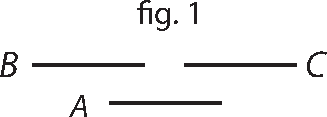
\includegraphics[width=0.25\textwidth]{%
gesamttex/edit_VIII,3/images/LH_42_05_043_d1.pdf%
}%
\hfill%
\protect\raisebox{0.12em}{%
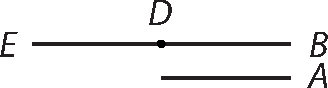
\includegraphics[width=0.25\textwidth]{%
gesamttex/edit_VIII,3/images/LH_42_05_043_d2.pdf%
}}
\hfill%
} % Hier leere Zeile

\vspace{0.5em}
\centerline{%
\hfill
\lbrack\textit{Fig.~1%,
}\rbrack %
\hspace*{45mm}
\lbrack\textit{Fig.~2%, 
}\rbrack
\hfill%
}
% \newpage%
\vspace{1.5em}
%
\pstart\noindent
%
Si \textit{A} simul incurrat in \textit{B} et \textit{C} eodem modo, tunc eodem modo perget, aut quiescet, aut reflectetur
%
ac si \textit{B} et \textit{C} essent connexa neque enim ulla est causa gyrationis%
\protect\index{Sachverzeichnis}{gyratio} in ipso.
%
Praeterea centrum commune gravitatis%
\protect\index{Sachverzeichnis}{centrum gravitatis commune} ipsorum \textit{B} et \textit{C} etiam eodem modo procedet, ac si essent connexa. 
%
Postremo corpus \textit{B} eodem modo movetur ut corpus \textit{C}. Quaedam tamen non habentur determinata, 
%
\edtext{nempe cum}{\lemma{nempe}\Bfootnote{\textit{(1)}~quod sit centru \textit{(2)}~cum~\textit{L}}}
%
%
%
corpora \textit{B} et \textit{C} utique gyrationem%
\protect\index{Sachverzeichnis}{gyratio} accipere oportent, quaeritur quod sit centrum gyri,%
\protect\index{Sachverzeichnis}{gyrus}\protect\index{Sachverzeichnis}{centrum gyri} et deinde 
%
quae proportio virium gyrationis%
\protect\index{Sachverzeichnis}{gyratio}%
\protect\index{Sachverzeichnis}{vis gyrationis} ad vires progressionis.%
\protect\index{Sachverzeichnis}{progressio}%
\protect\index{Sachverzeichnis}{vis progressionis} 
\pend 
%
\pstart
Si in fig.~2. \textit{A} et \textit{B} concurrant itidem nulla
%
\edtext{erit ipsius}{\lemma{erit}\Bfootnote{\textit{(1)}~communicatio \textbar\ ipsius \textit{streicht Hrsg.} \textbar\ \textit{A} \textit{(2)}~ipsius~\textit{L}}}
%
\textit{A} gyratio.%
\protect\index{Sachverzeichnis}{gyratio} 
%
Si \textit{A} pertingat ultra
%
\edtext{\textit{D}}{\lemma{}\Bfootnote{\textit{D} \textit{erg.~L}}} 
%
medium ipsius \textit{B}, manifestum est gyrationem\protect\index{Sachverzeichnis}{gyratio} fieri non posse circa medium ipsius \textit{B}. 
%
Si \textit{A} praecise occupet \edtext{\textit{DB}\lbrack,\rbrack}{%
\lemma{}%
\Bfootnote{%
\textit{DB} %
\textit{erg.~L}%
}}
unam medietatem ipsius \textit{B}, quaeritur an tunc %
gyratio\protect\index{Sachverzeichnis}{gyratio} fiat circa \textit{D} 
%
punctum medium%
\protect\index{Sachverzeichnis}{punctum medium} ipsius \textit{B}. Quaeritur et an 
%
\edtext{idem fiat}{\lemma{idem}\Bfootnote{\textit{(1)}~sit \textit{(2)}~fiat~\textit{L}}}
%
sive corpus \textit{A} feriat \textit{DBE}, vel \textit{DB} in \textit{DBE}, sive ejus loco aliud corpus redactum  
%
in ejus %
centrum gravitatis\protect\index{Sachverzeichnis}{centrum gravitatis} feriens \textit{DB} in medio, ita eodem modo ut \textit{A}. Ita suspicor. 
\pend 
%
\pstart
An licebit fingere initio adesse \textit{DB}, mox statim post intervallum temporis exiguum
%
addi \textit{ED}. Si haec via procederet haberetur solutio. 
\pend 
\count\Afootins=1200%
\count\Bfootins=1200%
\count\Cfootins=1200